%!TEX root = ../memoire.tex

\chapter{Génération automatique de texte}

%%%%%%%%%%%%%%%%%%%%%%%%%%%%%%%%%%%%%%%%%%%%%%%%%%%%%%%
% --------- I N T R O   ---------
%%%%%%%%%%%%%%%%%%%%%%%%%%%%%%%%%%%%%%%%%%%%%%%%%%%%%%%

La \acf{GAT} découle de la branche qu'est le \acf{TAL}. Reiter et Dale  définissent cette branche comme étant un domaine à la croisée des chemins entre l'intelligence artificielle et la linguistique computationnelle \citep{ReiterBuildingNaturalLanguage2000}. L'objectif de la \ac{GAT} est de développer des sytèmes pouvant produire du texte compréhensible en langue naturelle à partir de données (non-linguistiques). Bien que cet objectif soit commun à tous les générateurs de texte, il existe diverses méthodes pour l'achever. La diversité des méthodes est une conséquence directe des divers types d'input possibles (données non-linguistiques, texte et des images \citep{thomason:coling14}) et des diverses approches pour réaliser l'output (à base de patrons, à base de règles, stochastiques \citep{gatt18}).

Toutefois, avant d'entrer dans les détails de la \ac{GAT}, il serait pertinent de présenter l'origine de ces systèmes. À la base, ils ont été conçus pour, entre autre, générer des rapports automatiquement afin de faciliter le travail des êtres humains \citep{ReiterBuildingNaturalLanguage2000}. À ce sujet, Daoust et Lapalme soutiennent que\cite{DaoustJSREALTextRealizer2015} la \ac{GAT} nous permet de générer un résumé d'information provenant d'un input numérique qui est incompréhensible pour un humain. D'ailleurs, en plus de fournir des résumés automatiques, ces systèmes de \ac{GAT} opèrent les tâches sans se fatiguer. Ces tâches automatiées permettent d'éviter des coûts en termes de ressources et de temps. De plus, les textes générés automatiquement n'ont pas besoin d'être lus par une quantité phénomènale de gens pour être considérés utiles. Dès qu'ils remplissent leur fonction auprès d'une poignée de gens, leur raison d'être est justifiée. On est même capable de générer du texte en fonction du lecteur. Ainsi, on pourrait générer un rapport quelconque en fonction du niveau de compréhension des données. Par exemple, un professionnel, un technicien ou un client \citep{1948c0b7a8ca42679cad977bb2cdddc2} ne se ferait pas offrir le même rapport. La \ac{GAT} a aussi fait son émergence dans le robo-journalisme. Par exemple, lorsqu'un matchs sportif ne bénéficie pas de couverture médiatique, on peut fournir les données brutes du match (qui a compté, à quelle minute, les fautes, etc.) à un système de \ac{GAT} et il en sortira un résumé du match en langue naturelle \citep{W17-3513}.

Il est aussi important de préciser que la \ac{GAT} présente une valeur linguistique théorique. En effet, de nombreux linguistes ont testé leurs théories en développant des générateurs automatique de texte pour vérifier si leur modélisation de la langue fonctionnait dans un système computationnel \citep{DanlosPresentationmodelegeneration1983}. 

Depuis que Dale et Reiter ont publié leur livre \citep{ReiterBuildingNaturalLanguage2000}, le domaine a subi quelques changements. Avec l'émergence des méthodes statistiques, on fait maintenant de la génération de texte automatique en prenant des images comme input\citep{DBLP:journals/corr/HendricksARDSD16}. De plus, les frontières entre les diverses approches s'affaissent avec le temps. Conséquemment, nous sommes témoins d'une émergence continue de systèmes hybrides. Par exemple, des systèmes à base de règles utilisant des méthodes statistiques pour combler certaines tâches \citep{gatt18}. C'est un domaine en constante évolution.

Dans le cadre de ce mémoire, nous élaborerons plus précisément sur une partie du processus de la \ac{GAT}: la réalisation. Cependant, avant de décrire cette étape, nous allons jeter les bases de la \ac{GAT} en décrivant le pipeline classique.

%%%%%%%%%%%%%%%%%%%%%%%%%%%%%%%%%%%%%%%%%%%%%%%%%%%%%%%
% --------- P I P E L I N E   ---------
%%%%%%%%%%%%%%%%%%%%%%%%%%%%%%%%%%%%%%%%%%%%%%%%%%%%%%%

\section{Pipeline classique GAT} \label{ppc}

. Traditionnellement, la \ac{GAT} est un processus séquentiel séparé en diverses sections. Selon Dale et Reiter \cite{ReiterBuildingNaturalLanguage2000}, les six étapes suivantes sont celles qui composent normalement un système de génération. Nous les illustrons à la figure~\ref{fig:Pipeline}.
%les figures latex bougent, donc évite les formulations comme ça.
\begin{figure}[htb] % utilise toujours [htb]
	\centering
	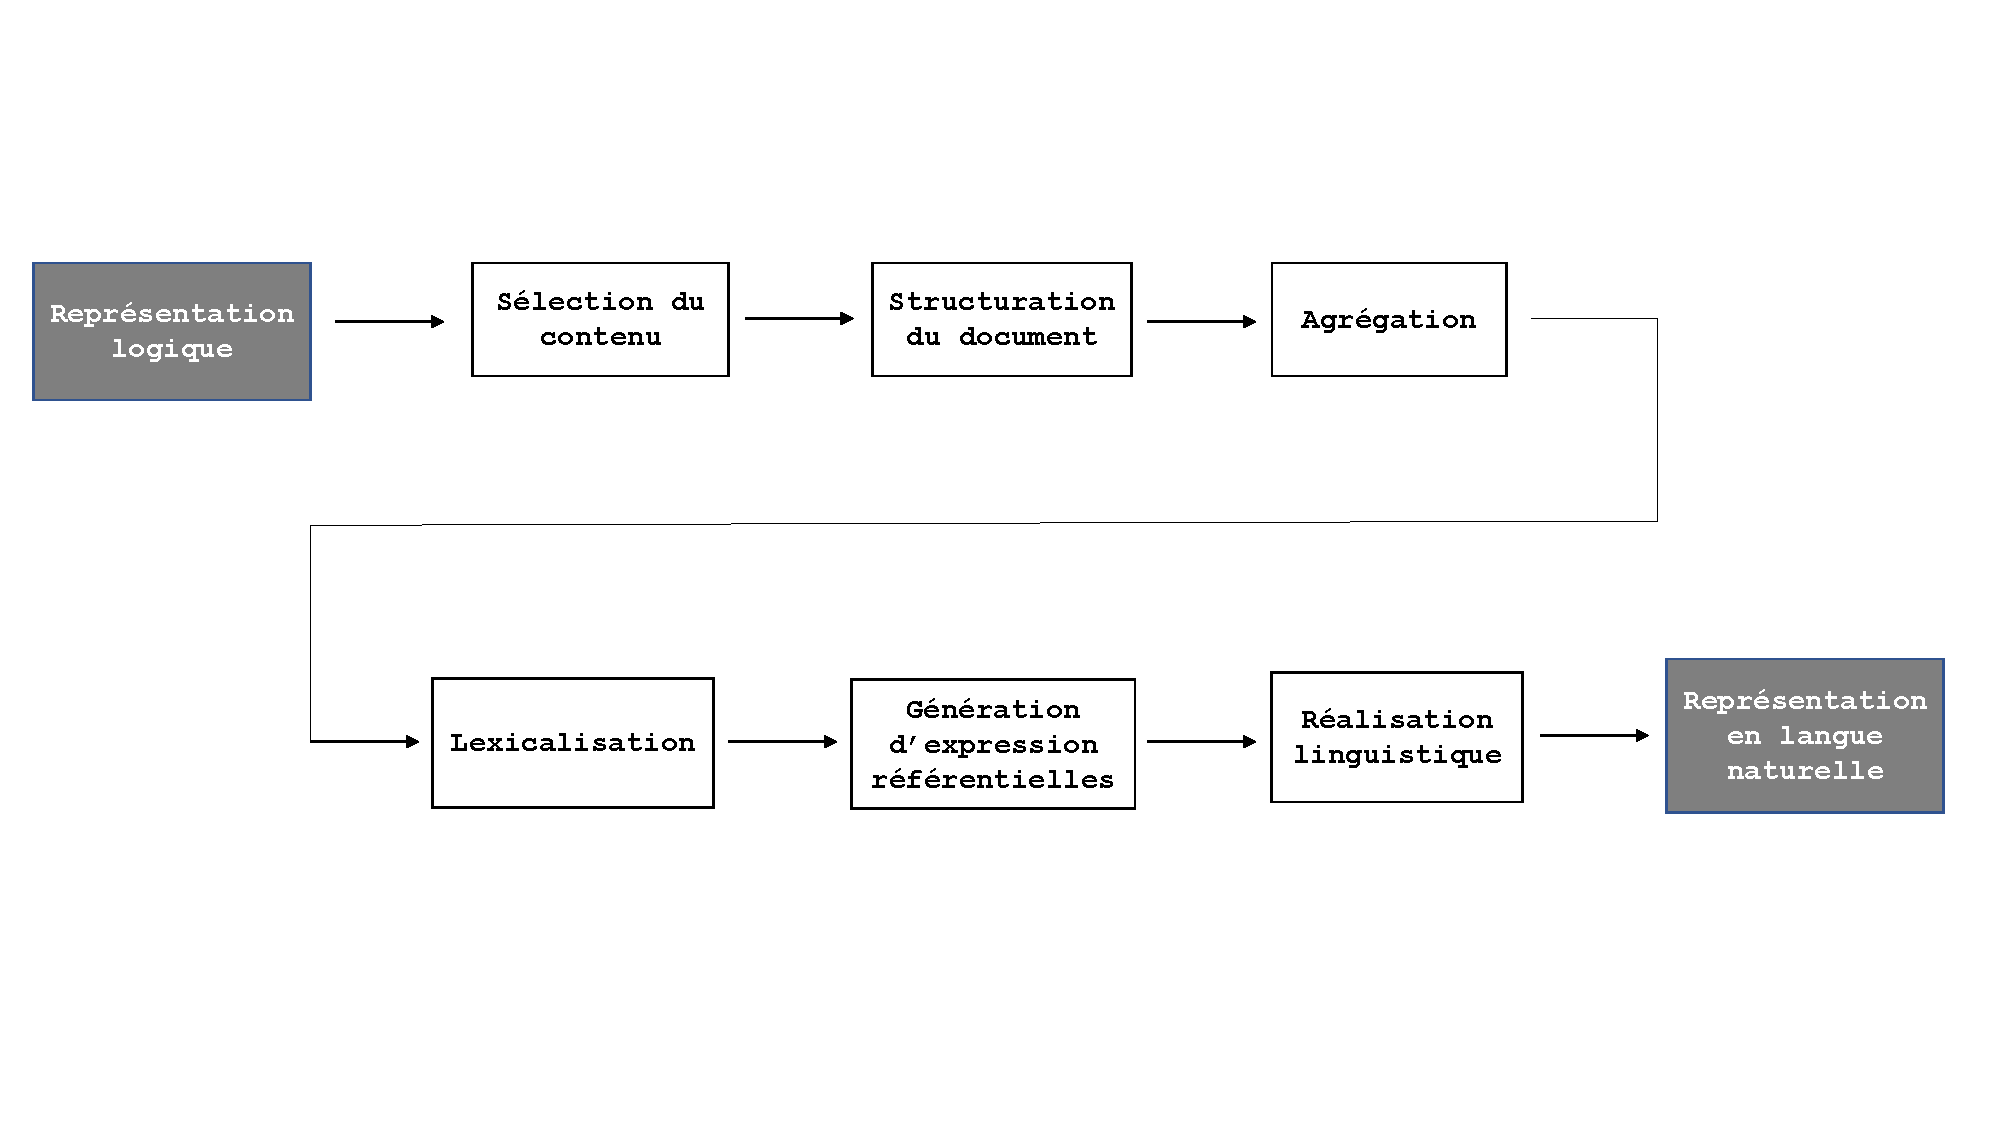
\includegraphics[width=1\textwidth, trim = {0cm 0cm 0cm 0cm},clip]{ch2/figs/pipeline.pdf}
	\caption{Pipeline classique}
	\label{fig:Pipeline}
\end{figure}

\draft{reformuler ce paragraphe}Beaucoup s'entendent pour dire qu'il y a deux parties à la \ac{GAT}. Le \emph{quoi-dire} et le \emph{comment-le-dire} selon \citep{DanlosPresentationmodelegeneration1983}, puis le \emph{early process} et le \emph{late process} selon \citep{gatt18}. Le quoi-dire correspond au early process et le comment-le-dire fait référence au late process. La premier fait référence à la sélection du contenu,la structuration de celle-ci et l'agrégation, puis le second fait référence à toutes les étapes subséquentes : la lexicalisation, la génération d'expressions référentielles et la réalisation linguistique. Pour mieux comprendre le processus de \ac{GAT}, nous décrirons en quelques lignes chacune des étapes qui la compose.

\subsection{Sélection du contenu}
Un système de \ac{GAT} doit départir les informations qui figureront dans le texte de celles qui n'y seront pas. La sélection du contenu dépend de l'objectif de la tâche. Par exemple, si un texte s'adresse à un débutant le niveau de détails du contenu à rendre devra correspondre à l'utilisateur. Il faut donc faire des choix quand au contenu qui sera généré. Par exemple, s'il s'agit de données pour un match de soccer, on ne voudrait probablement pas réaliser en texte toutes les passes et les fautes commises durant le match même si ces informations figurent dans l'input.

\subsection{Structuration du document}
Après avoir sélectionné le contenu, un système de \ac{GAT} doit décider l'ordre dans lequel les informations sélectionnées seront présentées. Reprenons l'exemple du soccer. En fonctions des données choisies, le texte devrait débuter par les informations générales liées au match (où et quand le match s'est déroulé), suivi du noms des équipes qui s'opposaient, puis des points important en terminant par l'issue du match. Il s'agit de créer le plan du texte. Cette étape est une représentation ordonnée et structurée de messages à transmettre. 

\subsection{Agrégation}
L'agrégation est l'étape où on combine des messages en une seule phrase afin de rendre le texte plus fluide et agréable à lire. Les messages sélectionnés dans le plan (structuration du document) n'ont pas à être exprimé dans des phrases individuelles si on peut les combiner en une phrase \citep{ChengCapturingInteractionAggregation2000}. Bref, cette étape sert à rendre le texte moins redondant.

\subsection{Lexicalisation}
À cette étape, une bonne partie de la pré-production a été entamée, on peut commencer à traduire les données non-linguistiques en langue naturelle. Cette partie est très importante car on y sélectionne les mots qui seront utilisés pour transmettre le message. Comme il existe naturellement plusieurs manières pour traduire une même idée en mots, cette tâche peut devenir assez complexe si on veut que le système puisse tenir compte de la réalité du langage. La sélection des mots peut ainsi se faire à divers niveaux d'abstractions. Un niveau plus abstrait requière plus de travail et est plus complexe à mettre en place, mais génère plus de possiblités au moment de la réalisation. Elhadad \cite{ElhadadFloatingConstraintsLexical1997} postulait dès le début une approche en faveur de la lexicalisation profonde.

\subsection{Génération d'expressions réferentielles}
Cette opération est très similaire à la lexicalisation car on choisit comment se réaliseront certaines entités. On l'appelle "`l'étape discriminatoire"' car le but est de s'assurer que le lecteur puisse distinguer correctement chaque entité se trouvant dans le texte. Pour cela, il faut trouver la meilleure façon de référer à une entité.

\subsection{Réalisation linguistique}
La dernière étape est la réalisation linguistique. Lorsque tous les mots ont été choisis, puis successivement, toutes les phrases ont été planifiées, il faut les réaliser en texte final et grammatical. Cette tâche implique l'application de traits morpho-syntaxiques aux lexèmes et la linéarisation des structures. Elle inclut aussi l'insertion des mots fonctionnels (auxiliaires, déterminants,etc.) et la ponctuation.

À ce sujet, il existe plusieurs approches pour effectuer la réalisation linguistique. Nous les présentons brièvement ici.

\subsubsection{À base de patrons}
Cette approche est utilisée pour générer du texte dans des domaines précis (météo,sport) et dans lesquels les variations linguistiques réalisables sont minimisées \citep{mcroy_channarukul_ali_2003}. Les phrases en \ref{template} provenant de \cite{gatt18} démontrent comment les patrons s'utilisent.

\ex. \label{template} \emph{À base de patrons}
	\a.\$player scored for \$team in the \$minute minute. 
	\b. Ivan Rakitic scored for Barcelona in the 4th minute.

En \ref{template}, le patron contient trois variables marquées par les \$. Celles-ci peuvent être respectivement comblées par un nom de joueur, suivi d'un nom d'équipe et d'une indication temporelle. Cet exemple démontre bien l'avantage d'utiliser des réalisateurs à base de patrons. Ils permettent de prévoir ce qui sera généré en output et cela diminue les risques d'erreurs. Toutefois, puisqu'ils sont codés à la main, ces sytèmes ont l'inconvénient d'être coûteux en termes de temps. Les réalisateurs à base de patrons peuvent être complémentés par des règles de grammaire, ce qui les rend plus flexibles. Ils peuvent aussi être combinés à de l'apprentissage machine. Cela automatise l'écriture des patrons et rend la tâche moins coûteuse en termes de temps \citep{gatt18}.

\subsubsection{À base de règles grammaticales}
Les modèles à base de règles grammaticales s'emploient autant des les domaines spécifiques (météo, sport) que les domaines généraux (le parler quotidien). Effectivement, ils se prêtent bien à la réalisation de domaine général car ils ont comme fonction de pouvoir réaliser du texte de la manière la plus humaine et naturelle possible. La combinaison de règles de grammaire et de dictionnaires mèneront à la bonne formation de phrases. Cependant, les grammaires et dictionnaires sont codés manuellement, ce qui demande du temps et des ressources.

\subsubsection{Statistiques}
\draft{relire}Il existe divers emplois des méthodes statistiques. On peut l'utiliser pour filtrer les ouputs dans un système où les statisitques détermineront quel output est le meilleur candidat \citep{LangkildeForestbasedStatisticalSentence2000}, approche \emph{generate-and-filter}. Dans cette approche on utilise encore un noyau de règles manuellement encodées. Toutefois, il existe aussi des approches statistiques de réalisation n'utilisant pas de noyau de règles manuellement encodés. Les règles sont apprises automatiquement par apprentissage machine avec de large corpus (white et rajkumar 2012). Cela diminue considérablement la charge de travail manuelle.

\subsubsection{Règles versus statistiques : avantages/inconvénients}

\draft{relire}Maintenant que nous avons présenté ces approches, nous nous posons la question:"' Est-ce que l'encodage manuel est toujours pertinent à l'ère des méthodes statistiques"'. Traditionnellement, les systèmes de \ac{GAT} tendaient vers des ressources encodées manuellement. Mais, de tels ressources nécessitaient du temps (et des ressources). Cela a poussé plusieurs chercheurs à automatiser la réalisation linguistique \citep{LangkildeForestbasedStatisticalSentence2000}.\cite{BelzSystemBuildingCost2009} s'est penché sur cette question dans son article. Concrètement, elle se demandait si le temps qu'on gagne en automatisant la réalisation se fait au détriment de la qualité de celle-ci. Si c'est le cas, à quel point la qualité de l'output est affectée. Elle a évalué une tâche de réalisation en utilisant un système à base de règles, puis un système statistique. L'évaluation se faisait en deux temps. D'abord une évaluation humaine pour traiter la qualité des outputs des deux systèmes, puis une évaluation métrique faite. Après l'évaluation, Belz nous explique que les évaluations humaines pointaient en faveur des systèmes à base de règles. De plus, elle suggère que certaines évaluations métriques surévaluent parfois les systèmes statistiques et sous-évalue les systèmes manuels\citep{BelzSystemBuildingCost2009}. 

\draft{relire}Reiter s'est aussi penché sur la question et il fait un survol du sujet dans son blog \cite{ReiterNaturalLanguageGeneration2016} \draft{vérifier comment citer un blog}. Selon lui, même si les systèmes d'apprentissage machine génèrent du bon texte la plupart du temps, ils peuvent occasionnellement générer du texte bizarre et inapproprié (et les évaluations sont souvent basés sur la moyenne du bon texte généré et pas par rapport aux incongruités générées). De plus, il souligne que lorsque des incongruités sont générées, les systèmes basés sur des méthodes statistiques ont plus de difficultés à les corriger car le tout est basé sur les statistiques. En contre partie, les systèmes à base de règles où permettent de cerner le problème avec plus de facilité et le corriger. Ce comportement n'est pas approprié dans des domaines professionnels ou personnels où des utilisateurs comptent sur la qualité des textes générés automatiquement, entre autre, car ils prendront potentiellement des décisions en fonction de leur lecture. Cependant, Reiter termine son article de blog en soulignant que la \ac{GAT} a beaucoup à gagner des méthodes statistiques. Il suggère de se servir de celles-ci pour automatiser des composantes d'une approche à base de règles.

%%%%%%%%%%%%%%%%%%%%%%%%%%%%%%%%%%%%%%%%%%%%%%%%%%%%%%%
% --------- R É A L I S A T I O N   ---------
%%%%%%%%%%%%%%%%%%%%%%%%%%%%%%%%%%%%%%%%%%%%%%%%%%%%%%%


\section{Réalisation}

Notre projet consiste à doter un réalisateur profond d'un dictionnaire verbal riche pour lui permettre de couvrir toute la grammaire anglaise. Donc, pour une meilleure compréhension de la tâche qu'est la réalisation de texte, nous décrirons quelques réalisateurs brièvement.

Tel qu'explicité à la figure~\ref{fig:Pipeline}, la réalisation est la dernière étape dans le processus de \ac{GAT}. Toutefois, pour beaucoup de chercheurs, elle ne représente pas uniquement les tâches décrites précédemment. Il règne une ambiguité quant aux concepts qu'incarne la réalisation. Lambrey le mentionne \cite{LambreyImplementationcollocationspour2017} dans son mémoire, effectivement, le terme technique \emph{réalisation} peut faire référence, à la fois aux systèmes qui performent la tâche de réalisation linguistique telle que décrite dans le pipeline classique (figure \ref{ppc}), mais elle réfère aussi aux engins qui opèrent la réalisation ainsi que des tâches se trouvant en amont de la réalisation classique (notamment la lexicalisation). Nous utiliserons dans ce mémoire les mêmes disctinctions que \citep{LambreyImplementationcollocationspour2017}. Ainsi, on appellera un réalisateur de surface un engin qui s'occupe de la réalisation linguistique à un niveau plus superficiel, prenant comme input des structures syntaxiques dont les unités sont déjà lexicalisées. On appellera un réalisateur profond un système qui effectue la réalisation en partant d'un niveau plus abstrait, c'est-à-dire généralement un niveau sémantique et dont les unités ne sont pas lexicalisées dans l'input. Ces réalisateurs profonds nécessitent des dictionnaires explicitant la combinatoire des unités lexicales et des grammaires plus complexes afin de traiter l'interface sémantique-syntaxe. Ces systèmes sont généralement liés à une théorie linguistique permettant de modéliser l'interaction entre l'input, le dictionnaire, la grammaire et l'output.

%%%%%%%%%%%%%%%%%%%%%%%%%%%%%%%%%%%%%%%%%%%%%%%%%%%%%%%
% --------- R É A L I S A T E U R   S U R F A C E ---
%%%%%%%%%%%%%%%%%%%%%%%%%%%%%%%%%%%%%%%%%%%%%%%%%%%%%%%

\subsection{Réalisateurs de surface}

Parmi les premiers réalisateurs à base de règles, les choix qui mèneront à la génération de texte dépendent des unités lexicales et des règles de grammaires combinées. Ce qui nécessite que les systèmes sont codés très minutieusement, puisque les langues naturelles sont complexes et très riches. Ces systèmes exigent des niveaux de détails qui demande beaucoup de temps à créer et les rendant plus difficile à insérer dans le pipeline classique. C'est ce qui les distingue des réalisateurs profonds c'est qu'ils ne requièrent pas de théorie linguistique sous-jacente en raison de leur traitement du langage en surface. Les réalisateurs de surface sont généralement plus simples à utiliser et à implémanter dans un pipeline de \ac{GAT} \citep{gatt18} parce que les choix lexicaux et les structures syntaxiques ont déjà été effectué \citep{lareau18}. Les choix lexicaux étant déjà fait avant l'étape de réalisation, les réalisateurs de surface prennent en input une représentation syntaxique, donc lexicalisée. Dans ces systèmes, les dictionnaires et règles traitent l'interface morpho-syntaxique. Finalement, ils correspondent plus à la phase de réalisation mentionnée dans le pipeline classique de Dale et Reiter.

\subsubsection{SimpleNLG}
SimpleNLG est \citep{GattSimpleNLGRealisationEngine2009} est un réalisateur de surface écrit en java. Il opère une réalisation de surface à partir d'une structure syntaxique déjà lexicalisée encodée en XML. Par la suite, SimpleNLG opère les opérations morphologiques nécessaires (flexion, dérivation des mots, linéarisation, ajout d'auxiliaires, gestion de l'accord) puis linéarise le texte en sortie.

Le réalisateur est doté d'une grammaire et d'un dictionnaire. Ce dernier encode les propriétés syntaxiques et morphologiques. Le module grammaticale contient aussi de l'information de nature morpho-syntaxiques, il est composé de règles permettant de passer de l'interace syntaxique à l'interface morphologique.

SimpleNLG découpe son processus de réalisation en quatre étpaes. Premièrement, les lexèmes compris dans la structure d'input sont matchés avec l'entrée lexicale qui leur corresponde. Deuxièmement, il faut déterminer les traits lexicaux attachés à ces entrées. Puis, troisièmement, les lexèmes sont combinés entre eux pour former des syntagmes de plus en plus grand jusqu'à ce que l'entièreté de la phrase forme un syntagme. Finalement, ces syntagmes sont linéarisés puis les règles morphologiques s'appliquent pour obtenir les formes fléchies et éventuellement la phrase désirée en output.

Noter que SimpleNLG a été traduit dans plusieurs langues : espagnol, italien, et français, portugais (Mazzei et al., 2016, Ramos-Soto 2017, Vaudry et Lapalme 2013 ; Oliveira et Sripada)

\begin{lstlisting}[language=Xml, caption=Structure d'input dans SimpleNLG, label=simplenlg]
<Document>
  <child xsi:type="SPhraseSpec">
    <subj xsi:type="VPPhraseSpec" FORM="PRESENT_PARTICIPLE">
      <head cat="VERB">
        <base>refactor</base>
      </head>
    </subj>
    <vp xsi:type="VPPhraseSpec" TENSE="PRESENT" >
      <head cat="VERB">
        <base>be</base>
      </head>
      <compl xsi:type="VPPhraseSpec" FORM="PAST_PARTICIPLE">
        <head cat="VERB">
          <base>need</base>
        </head>
      </compl>
    </vp>
  </child>
</Document>
\end{lstlisting}
La figure \ref{simplenlg} permet de réaliser la phrase 'Refactoring is needed.'

\subsubsection{JSreal}
JSreal \citep{DaoustJSREALTextRealizer2015} qui est en fait JavaScript Realiser. C'est un réaliseur de texte orienté pour les programmeurs web. C'est un réaliseur de texte en français qui génère des expressions et phrases bien formées qui elles peuvent être formattées en HTML pour être exposé dans un fureteur. Il peut aussi s'employer seul à des fins purement linguistiques ou être intégéré dans des générateurs de textes. Les Specs de JSreal sont similaires à ceux de SimpleNLG.

Pour générer du texte JSreal prend en input des structures syntaxiques lexicalisées. La bonne construction de la phrase provient du fait que les constituants de les structures syntaxiques vont faire appel à des règles, qui elles opèrent la combinaison des syntagmes entre eux jusqu'à ce que la structure au complet ait été parsée. Pour générer du texte, JSreal possède les modules suivants : un dictionnaire et une grammaire (règles syntaxiques et morphologiques). Son dictionnaire défini la catégorie des mots qui le peuple, et les traits lexicaux attachés (genre, nombre, irrégularités, etc.). Les règles morpho-syntaxiques permettent de : .Il existe aussi une version bilingue de JSreal \citep{MolinsJSrealBBilingualText2015}.

\begin{lstlisting}[language=Xml, caption=JSreal, label=jsreal]
JSrealLoader({
        language: "en",
        lexiconUrl: URL.lexicon.en,
        ruleUrl: URL.rule.en,
        featureUrl: URL.feature
    }, function() {
    QUnit.test( "Sentence EN", function( assert ) {
        assert.equal(
            S(
                NP(D("the"), N("cat")),
                VP(V("sit"), PP(P("on"), NP(D("the"), N("coach")))).t("ps")
            )
        
\end{lstlisting}
La figure \ref{jsreal} produit la phrase :'The cat sat on the coach.'
		
\subsubsection{RealPro}
RealPro est implémenté en C++ \citep{LavoieFastPortableRealizer1997}. Il prend en input des arbres de dépendances.Le plus profond des réalisateurs de surface présénté jusqu'ici. La linéarisation s'opère entre le passage de la structure syntaxique de surface à la structure morphologique profonde. L'architecture de RealPro est basé sur la TST (citation). Brièvement, il s'agit d'une théorie qui schématise le langage en divers niveaux de représentations partant de la sémantique, syntaxe, morpho,phono, phoné. Ainsi, pour passer de la structure profonde à la strucutre de surface, le logiciel vérifie dans son dictionnaire (catégorie et information morphologique)et ses règles de grammaires pour s'assurer que le passage est grammatical. Ses connaissances lexicales sont encodées dans 2 modules: un dictionnaire et des règles de grammaires. Ceux-ci seront réquisitionnés par les diverses composantes au cours de la réalisation. Voici un graphique qui démontre leurs intéractions lors de la réalisation.
\begin{figure}[htb]
	\centering
	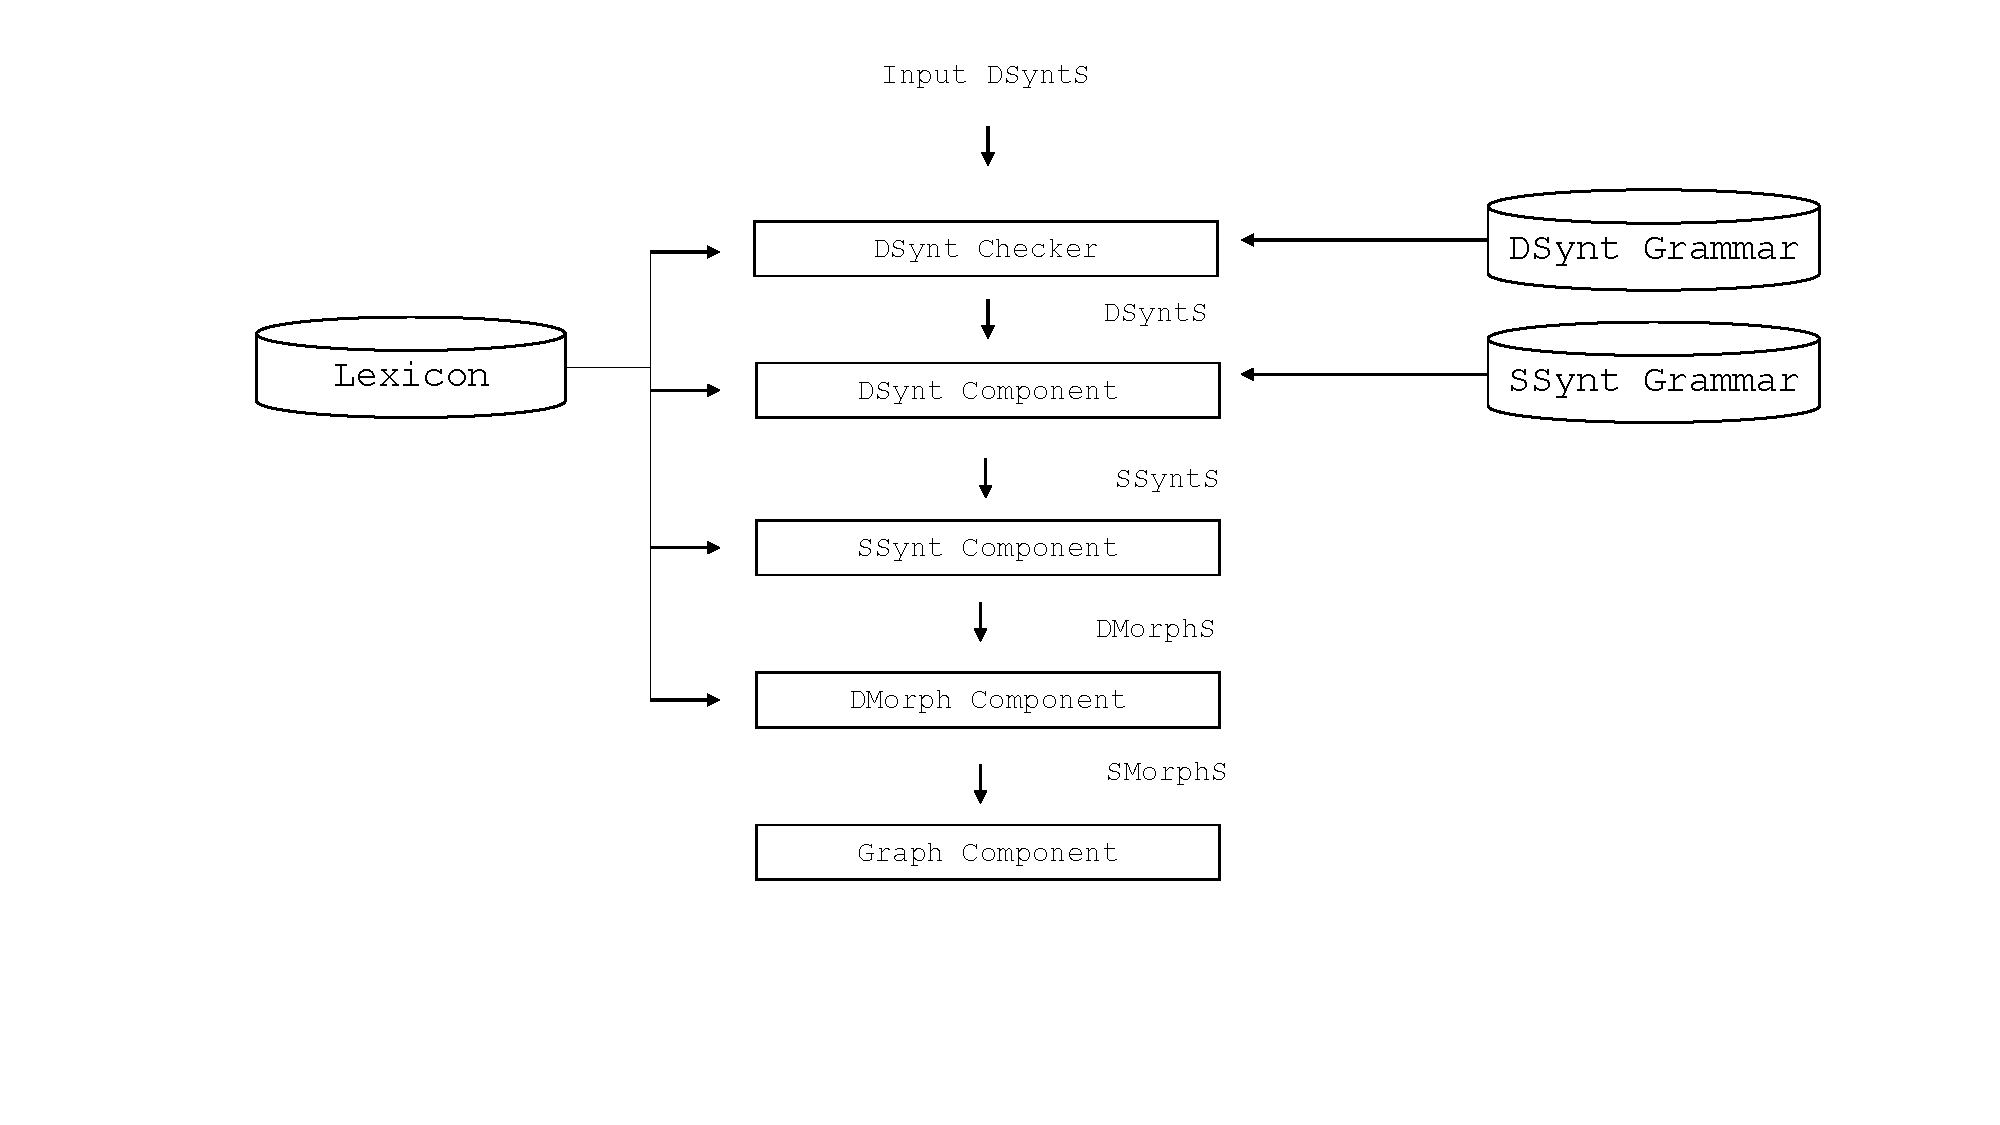
\includegraphics[width=1\textwidth, trim = {0cm 0cm 0cm 0cm},clip]{ch2/figs/realpro.pdf}
	\caption{RealPro}
	\label{fig:RealPro}
\end{figure}

\begin{lstlisting}[language=Xml, caption=Input, label=realpro]
HAVE1 [tense:past]
(I March [class:proper-noun]
II day [class:common-noun numberpl]
(ATTR rainy [class:adjective]))
\end{lstlisting}

Structure \ref{realpro} de dépendance représentant la phrase 'March had some rain days.'
%%%%%%%%%%%%%%%%%%%%%%%%%%%%%%%%%%%%%%%%%%%%%%%%%%%%%%%
% --------- R É A L I S A T E U R    P R O F O N D  ---
%%%%%%%%%%%%%%%%%%%%%%%%%%%%%%%%%%%%%%%%%%%%%%%%%%%%%%%

\subsection{Réalisateurs profonds}

Maintenant que nous avons exposé quelques générateurs de surface, nous exposerons des réalisateurs profonds. Généralement, ceux-ci sont construits autour d'une théorie linguistique sous-jacente afin de rendre compte des multiples phénomènes linguistiques plus profonds que permet l'interface morpho-syntaxique. Effectivement, on peut plus facilement construire un système profond en se basant sur un modèle théorique. Ces modèles permettent de prendre un input plus abstrait que les structures syntaxiques.

En prenant comme input des réseaux sémantiques on permet une plus grande flexibilité dans le contenu généré. Lorsque le choix lexical n'est pas encore fait au moment de la réalisation, il est encore possible de générer une même idée en différentes constructions. Dans le pipeline classique, la lexicalisation est opérée avant la réalisation, faisant en sorte que les inputs contiennent des lexèmes déjà choisis. Cela restreint le nombre de constructions possibles. Finalement, tel que Polguère le dit \cite{PolguerePourmodelestratifie}, si on veut un système qui génère du texte de la manière la plus naturelle possible, il faut qu'un réalisateur linguistique incorpore la lexicalisation. Lorsque la lexicalisation est traitée avant la réalisation, on impose en quelque sorte les réalisations possibles puisque le lexème a des contraintes. En prenant un lexème comme entrée, il vient avec toutes ses restrictions. Tandis qu'en prenant une unité sémantique, on peut la lexicaliser de manières différentes, donc cela créera des structures syntaxiques nécessairement différentes. D'où la flexibilité.  Les structures lexicalisées sont plus rigides et moins flexibles car pour être lexicalisées, il faut que la structure syntaxique soit déjà présente pour supporter les lexèmes. Si on prend un input plus abstrait, on n'a pas de structures pré-déterminées et on peut réaliser une idée de manières multiples. En fonction du choix des mots qui sera opéré.

\subsubsection{KPML}
KMPL\citep{BatemanEnablingTechnologyMultilingual1997} est un réalisateur linguistique multilingue issu du système PENMAN \citep{PenmanOverview}. C'est un système basé sur la grammaire fonctionnelle systémique (SFG) \citep{MatthiessenSystemicfunctionalgrammar1997}. Dans cette théorie, \draft{chaque choix linguistique est motivé par l'accomplissement d'une fonction. Cette perspective fonctionnaliste alimente l'aspect multilingue de KPML : les différentes langues partagent un certain nombre de fonctions. Seule la réalisation linguistique des fonctions diffère d'une langue à l'autre }.

\draft{La grammaire de KPML est encodée comme un réseau de système orienté (lisible de gauche à droite). Chaque intersection représente un choix grammatical minimal entre différents traits fonctionnels. Plus on avance dans le graphe, plus les choix deviennent spécifiques et précis. Cette architecture en réseau couvre tous les aspects linguistiques (phonologie, morphologie, syntaxe, etc.).}

Les structures d'input de ce système peuvent être de divers ordres: sémantiques et syntaxiques. Courte explication de la SFG : ressemble à la TST. Dans ce formalisme, la forme de surface est la conséquence directe de la sélection d'un ensemble de traits fonctionnels abstraits à partir d'une description des ressources du langage. Ces ressources sont représentées par des réseaux systémiques et dans ce formalisme la réalisation linguistique se fait en traversant les réseaux.

KPML prend des SPL en entrée. Il s'agit d'un acronyme pour \emph{Sentence Planning Language}. Un SPL est une matrice dont les objets sont des attributs et leurs valeurs.
\draft{Il traverse ses réseaux et produit un ensemble de déclarations de réalisation qui caractérisent le texte à générer, ces déclarations s'instanciant par des contraintes sur la forme grammaticale de la phrase. Ces contraintes sont spécifiées sous forme de matrices de traits grammaticaux. KPML arrive donc à généraliser beaucoup de phénomènes linguistiques grâce à ces réseaux.}

Afin d'illustrer à quoi ressemble l'input, nous allons reprendre un exemple de Dalet et Reiter: 'March had some rainy days'.
\begin{lstlisting}[language=Xml, caption=SPL: input de KPML, label=kpml]
(S1 \ generalized-possession
  :tense past 
	:domain (N1 \ time-interval
	            :lex march
							:determiner zero)
	:range (N2 \ time-interval
	           :number plural
						 :lex day
						 :determiner some
						 :property ascription
						 (A1 \ quality :lex rainy)))
\end{lstlisting}

\subsubsection{Surge}
\citep{Elhadad98surge:a}
Surge, qui signifie \emph{Systemic Unification Realisation Grammar of English}, est une grammaire de l'anglais. Elle est écrite en FUF\emph{Functional Unification Formalism} qui est basé sur FUG \citep{KayFunctionalUnificationGrammar1984}. FUF est un langage de programmation créé pour construire des grammaires computationnelles, plus particulièrement pour les besoins de la réalisation linguistique dans un cadre de grammaire d'unification. \draft{Son fonctionnement se base sur l'unification de graphes pour combiner une structure d'entrée (spécification de phrase) avec une grammaire de la langue de sortie. Le résultat est une structure spécifiée syntaxiquement qui est par la suite linéarisée pour produire la phrase finale.}

\draft{FUF prend en entrée des descriptions fonctionnelles (FD) décrivant le sens d'une phrase et une grammaire (aussi décrites en descriptions fonctionnelles). Ces descriptions fonctionnelles apparaissent sous la forme de matrices attributs-valeurs enchâssées. Le format de sortie est une phrase en anglais exprimant le sens voulu et suivant les normes grammaticales décrites par la grammaire}

Ils se servent de graphes d'unification comme input à leur système. Cet input est sous forme de FD (Functional Description), il s'agit d'une collection de paires attributs-valeurs dont l'union fournit une spécification de l'énoncé à génerer.

Nous reprendrons encore un exemple tiré de Dale et Reiter: 'March had some rainy days'.
\begin{lstlisting}[language=Xml, caption=FD: input de Surge, label=surge]
((cat clause)
 (proc ((type possessive)))
 (tense past)
 (partic ((possessor ((cat proper) head ((lex "March"))))
					(possessed ((cat common) head ((lex day)))
											(describer ((lex rainy)))
											(selective yes) (number plural)))))
\end{lstlisting}

Contrairement aux autres réalisateurs présentés ici, FUF n'utilise pas de dictionnaires, l'information lexicale est encodée dans la structure d'input.\draft{Le processus de réalisation profonde s'effectue en deux étapes. La première consiste à unifier les descriptions fonctionnelles du sens de la phrase à générer, c’est-à-dire enrichir la structure d’entrée, avec les spécifications syntaxiques et morphosyntaxiques de la grammaire. Ces spécifications permettent de gérer l'ordonnancement des mots, les constructions syntaxiques, l'accord, etc. Une fois l'unification terminée et la structure d'entrée enrichie, FUF linéarise la structure pour obtenir une phrase et prend en charge les contraintes morphologiques.}

\subsubsection{FORGe}
FORGe est un transducteur de graphes qui génère du texte à l'aide de ressources lexicales dictionnairiques et grammaticales \citep{MilledemoFORGePompeu2017}. C'est un réalisateur profond qui hérite de l'architecture de MARQUIS \citep{WannerMARQUISGENERATIONUSERTAILORED2010}. Nous décrirons ce réalisateur à la section \ref{sectionmarquis}  Il prend en entrée des représentations abstraites. Le système a été conçu pour l'anglais à la base, mais il se veut multilingue (espagnol, allemand, français et polonais sont en développement). C'est un système qui se base sur la théorie sens-texte \citep{melcuk1988}.

Input: représentations sémantiques en graphes acycliques composées de relations prédicats-arguments. Un exemple de ce type de graphe est fourni dans la figure \ref{fig:marquis} à la structure \#2 sémantique. 

Génération de structures syntaxiques profonds: Dans ce système, la structure syntaxique et la lexicalisation se font en même temps pour s'assurer que la structure résultante est conforme aux règles grammaticales et aux contraintes lexicales. Ainsi, les noeuds syntaxiques sont étiquettés par une partie de discours, et lors du passage de la sémantique à la syntaxe, on vérifie que le lexème qui consommera le noeud correspond à la partie du discours requise par ce noeud. De cette manière, FORGe construit un arbre de dépendance via un parsing successif du haut vers le bas. Ainsi, le noeud est lexicalisé et la structure des dépendants syntaxiques est créé en même temps, puis on vérifie que la partie du discours attribuée aux noeuds des dépendants correspond au lexème choisi par le système pour que ce soit une arbre de bonne forme. L'opération est effectuée successivement jusqu'à ce que toute la représentation sémantique ait été analysée. Il s'agit là du passage de la sémantique à la syntaxe, et il se fait via la combinaison des règles de l'interface en question et du dictionnaire.

Passage de la représentation sémantique à la structure syntaxique profonde via un parsing récursif top-down. Le top étant la racine syntaxique de la structure en développement, et une fois que le top est lexicalisé en syntaxe, on crée la structure qui lie ses dépendants syntaxiques, et les dépendants syntaxiques de ceux-ci jusqu'à ce qu'on parse la représentation sémantique au complet.

Ensuite, le passage de la syntaxe profonde à la syntaxe de surface(toujours des arbres de dépendances) où on introduit les mots fonctionnels (prépositions, auxiliaires, déterminants). Cette étape est possible grâce à la complexité des dictionnaires qu'ils utilisent. Par exemple, pour réaliser la bonne préposition en surface, ils ont implémenté un dictionnaire de valence à leur système. 

Finalement, la dernière étape consiste à appliquer les règles morpho-syntaxiques aux lexèmes et linéariser la structure syntaxique de surface.

pipeline multilingue et flexible: S'adaptent à différents type d'input assez facilement. Premièrement, la preuve a été fournie lors de la compétition SemEval 2017 où ils ont adapté leur format d'input à celui requis par la compétiton, ça ne leur a pris qu'une semaine \citep{DBLP:conf/semeval/MilleCBW17}. C'est un réalisateur qui peut aisément générer du texte en différentes langues grâce à ses règles grammaticales qui sont majoritairement language-independent. Les autres règles qui sont propres à l'anglais peuvent aisément être adaptées à d'autres langues. En conclusion, avec des ressources lexicales riches, on peut générer du texte dans plusieurs langues en peu d'efforts. D'ailleurs, les auteurs mentionnent que certains modules du systèmes peuvent être complémentés avec des méthodes statisitques, ce qui lui donne la possibilité de couvrir plus large.

\subsubsection{MARQUIS} \label{sectionmarquis}

Contrairement aux autres systèmes présentés ici, MARQUIS n'est pas qu'un réalisateur profond. Il s'agit d'un système de \ac{GAT} qui effectue toutes les étapes du processus de génération automatique de texte (section \ref{ppc}). Cependant, nous ne nous intéresserons qu'à l'aspect réalisation profonde de MARQUIS, pour plus d'informations, nous vous réferons à l'article \citep{WannerMARQUISGENERATIONUSERTAILORED2010}. 

MARQUIS est ainsi un projet dont le but est de générer à partir de données des bulletins météorologiques multilingue sur la qualité de l'air. Ces bulletins sont générés en fonction de l'utilisateur. Ainsi, la personne qui fait la requête d'un tel rapport entre ses informations personnelles et le bulletin sera générée en fonction de son expertise et de ses conditions médicales. Ainsi, un non-expert asthmatique se verra offrir un bulletin en fonction pouvant être lu par un non-expert et les données seront orientées en fonction de sa condition physique. Dans le cadre de ce travail, la partie qui décide le quoi-dire ne sera pas décrite ici. On décrira plutôt comment le système procède à la réalisation du message sélectionné par l'utilisateur.

MARQUIS est aussi un système basé sur la Théorie Sens-Texte, comme FORGe et RealPro. La réalisation profonde y est structurée de la même manière qu'on l'a expliqué avec FORGe, mais elle compte un niveau de profondeur de plus. Effectivement, MARQUIS étant un générateur multilingue (l'anglais, l'allemand, l'espagnol, le catalan, le portugais, le français, le finnois et le polonais.), le niveau de profondeur commun à toutes les langues du système et le niveau conceptuel. Celui-ci est encodé en graphes conceptuels et il forme un interface conceptuelle-sémantique avec le niveau sémantique. L'étape de réalisation profonde est ainsi la même que nous avons décrit avec FORGe, avec la particularité que MARQUIS ne fait pas appel à un dictionnaire de valence (il a donc moins de couverture). Afin de mieux expliciter la chose, la figure \ref{marquis} démontre bien comment ce système fonctionne.

MARQUIS part de la représentation conceptuelle qui passe par les niveaux de représentations jusqu'au texte.

\begin{figure}[htb]
	\centering
	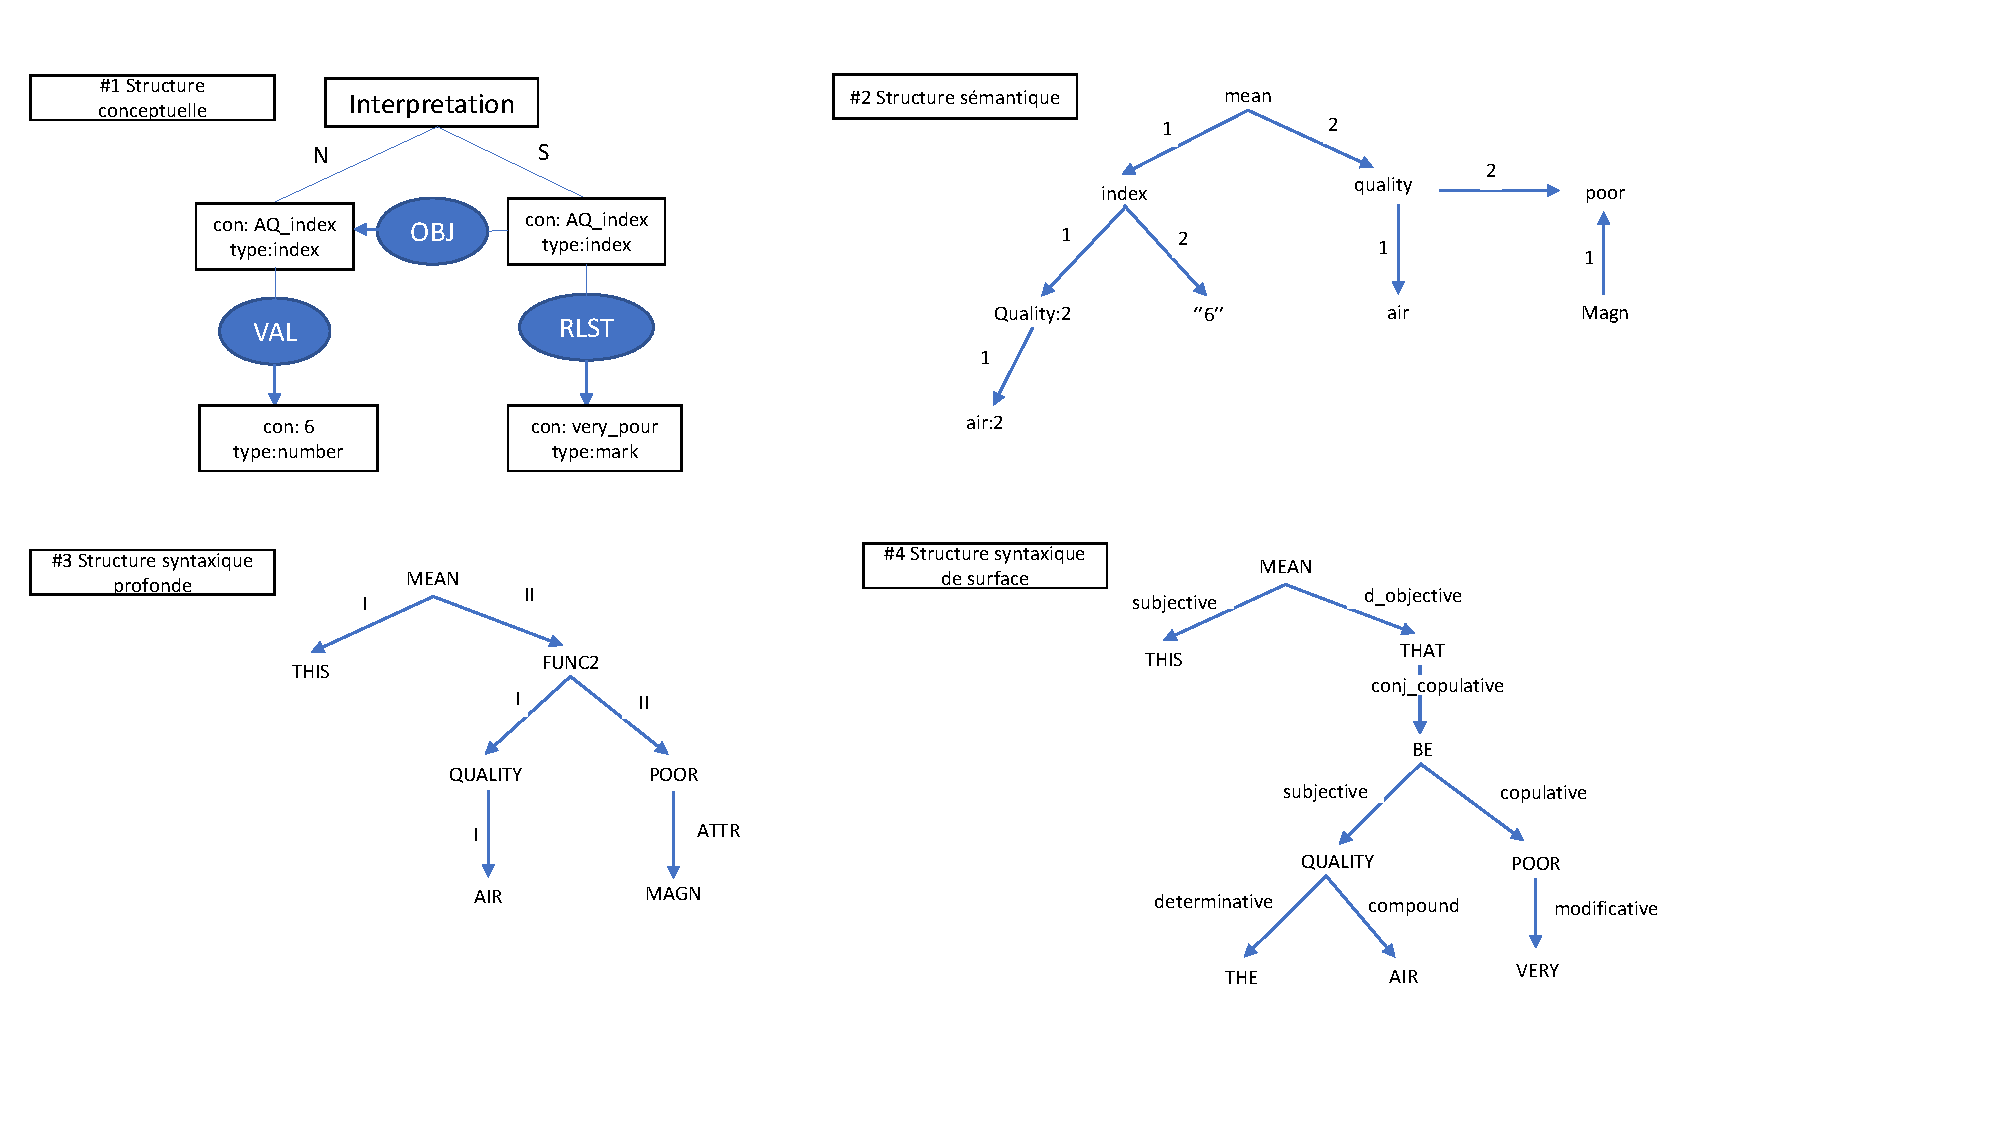
\includegraphics[width=1\textwidth, trim = {0cm 0cm 0cm 0cm},clip]{ch2/figs/marquis.pdf}
	\caption{Pipeline de MARQUIS}
	\label{fig:marquis}
\end{figure}

Pour résumé cette figure,
Prend en input : graphes conceptuels 
rend en output : du texte
entre les 2 : séries de dérivations (changements successifs de représentations en fonction des divers niveaux de représentations. ce qui assure la grammaticalité des changements est : l'information lexicale encodée dans les dictionnaires et les modules de règles qui modélise chaque interface).

Par exemple, voici comment les dictionnaires et règles fonctionnent \draft{reprendre la figure 11 de Florie}
Le dictionnaire conceptuel comprend tous les concepts utiles à la génération des rapports sur la qualité de l'air et les autres termes généraux du langage. Puis il mappe les concepts aux unités sémantiques (dans chaque langue) qui leurs correspondent. Le dictionnaire sémantique contient les unités sémantiques. Une même unité sémantique peut être réalisée par deux lexèmes différents. Ainsi, il nous faut un dictionnaire lexémique qui contient toutes les unités lexicales et leurs traits. Par la suite, une fois que les unités sont lexicalisées, nous n'avons plus besoin d'autres dictionnaires. 

Tel que démontré, MARQUIS et FORGe partent de niveaux d'abstraction plus profond que les autres systèmes présentés. Cela leur permet d'être beaucoup plus flexible dans leur réalisation linguistique. C'est pourquoi nous utilisons aussi un réalisateur profond doté de paramètres très similaires à ces deux réalisateurs. Comme FORGe, nous utiliserons aussi un système basé sur MARQUIS. Il s'agit de GenDR \citep{lareau18}: un projet en cours de développement dirigé par François Lareau à l’Observatoire de linguistique Sens-Texte. Le chapitre suivant décrira en détails ce réalisateur.